\documentclass[fleqn,10pt,a4paper,titlepage]{article}
\includeonly{common,feluletek,vektoranalizis}



%
% - ---- -- PACKAGES--------------------------
%

\usepackage{amssymb}
\usepackage{amsmath}
\usepackage[T1]{fontenc}
\usepackage[utf8]{inputenc}
\usepackage[magyar]{babel}
%\usepackage{amsthm}
\usepackage{theorem}
\usepackage{fancyhdr}
\usepackage{lastpage}
\usepackage{paralist}
\usepackage{enumerate}

%
% ---------- CODES --------------------------
%
\makeatletter
\gdef\th@magyar{\normalfont\slshape
  \def\@begintheorem##1##2{%
  \item[\hskip\labelsep \theorem@headerfont ##2.\ ##1.]}%
  \def\@opargbegintheorem##1##2##3{%
  \item[\hskip\labelsep \theorem@headerfont ##2. ##1.\ (##3)]}}
\makeatother


%
% ------------  N E W  C O M M A N D S --------
%


\theoremstyle{magyar}
\theoremheaderfont{\itshape\bfseries}
\newtheorem{de}{definíció}[section]
\newtheorem{te}{tétel}[section]
\newtheorem{bi}{bizonyítás}[section]
\newtheorem{ko}{következmény}[section]
\newtheorem{me}{megjegyzés}[section]
\newtheorem{al}{állítás}[section]

%
% ------- S E T T I N G S ----------------
%

\newcommand{\mktoc}{
  \pagenumbering{roman}
  \setcounter{page}{1}
  \lhead{\textbf{\thepage}}
  \cfoot{}
  \tableofcontents
  \newpage
  \lhead{\textbf{\thepage}}%/\pageref{LastPage}}
  \pagenumbering{arabic}
  \setcounter{page}{1}
}

\usepackage{booktabs}
%\usepackage{epsfig}
%\usepackage{psfrag}
%\usepackage{graphics}


\newcommand{\eqrho}{\stackrel{\varrho}{=}}
\newcommand{\eqrhon}[1]{\stackrel{\varrho_{#1}}{=}}
\newcommand{\MT}{\ensuremath{(M,\varrho)}\,}
\newcommand{\MTn}[1]{\ensuremath{(M,\varrho_{#1})}\,}
\newcommand{\sorozat}{\ensuremath{(a_n)\colon \N\n M}\,}
\newcommand{\sorozatn}[1]{\ensuremath{(a_{#1})\colon \N\n M}}

\renewcommand{\sectionmark}[1]{\markboth{\Roman{section}. fejezet\\#1}{}}
\newcommand{\hullam}{\widetilde}
\newcommand{\mr}[1]{(M_{#1},\,\ro_{#1})}
\newcommand{\fmm}{f\in M_1\n M_2}
\newcommand{\X}{\ensuremath{\mathcal{X}}}
\newcommand{\lp}{\ensuremath{l_p}}
\newcommand{\norma}[1]{\ensuremath{\left\Vert #1\right\Vert}}
\newcommand{\norman}[2]{\ensuremath{\norma{#1}^{(#2)}}}
\newcommand{\Norma}{\norma{\cdot}}
\newcommand{\Norman}[1]{\ensuremath{\Norma^{(#1)}}}
\newcommand{\opnorma}[1]{\ensuremath{|||#1|||}}
\newcommand{\NT}{\ensuremath{(\X,\,\Norma)}}
\newcommand{\skalar}[2]{\ensuremath{\langle#1,\,#2\rangle}}
\newcommand{\Skalar}{\skalar{.}{.}}
\newcommand{\skalarsz}{\Skalar}
\newcommand{\ET}{\ensuremath{(\X,\,\skalarsz)}}
\newcommand{\nullelem}{\mathsf{0}}
%\renewcommand{\square}{\blacksquare}
\newcommand{\RnRm}{\R^n\to\R^m}
\newcommand{\RnRn}{\R^n\to\R^n}
\newcommand{\RnR}{\R^n\to\R}
\newcommand{\RRm}{\R\to\R^m}
\newcommand{\Rnrm}{\RnRm}
\newcommand{\Rnrn}{\RnRn}
\newcommand{\RRn}{\R\times\R^n}
\newcommand{\Linearis}{\ensuremath{\mathcal{L}(\R^n,\,\R^m)}}
\DeclareMathOperator{\intD}{int\,D}
\DeclareMathOperator{\Folyt}{C}
\newcommand{\folyt}[1]{\Folyt\{#1\}}
\newcommand{\derivp}[1]{\D\{#1\}}
\newcommand{\dern}[2]{\D^{#1}\{#2\}}
\newcommand{\der}[1]{\derivp{#1}}
\newcommand{\vekt}[1]{\mathbf{#1}}
\newcommand{\Rmn}{\ensuremath{\R^{m\times n}}}
\DeclareMathOperator{\grad}{grad}
\newcommand{\vfi}{\varphi}
\newenvironment{spec}{\begin{trivlist}\item\relax\mbox{\textbf{Spec. esetek.\enskip}}\ignorespaces}{\end{trivlist}}
\newtheorem{lemma}{lemma}[section]
\newtheorem{pelda}{PÉLDA}[section]
\DeclareMathOperator{\sgn}{sgn}
\DeclareMathOperator{\ch}{ch}
\DeclareMathOperator{\sh}{sh}
\DeclareMathOperator{\arctg}{arctg}
\newcommand*{\Der}{\D}
\newcommand*{\Oint}{\oint\limits}
\DeclareMathOperator{\Rint}{R}
\DeclareMathOperator{\re}{\Re e}
%\newcommand{\re}{\Re}
\DeclareMathOperator{\im}{\Im m}
%\newcommand{\im}{\Im}
\newcommand{\ERTT}{\mathcal{D}}
\newcommand{\fcc}{f\in\C\to\C}
\DeclareMathOperator{\fr}{fr}
\DeclareMathOperator{\intG}{int}
\DeclareMathOperator{\rang}{rang}
\DeclareMathOperator{\dist}{dist}
\DeclareMathOperator{\tr}{tr}
\DeclareMathOperator{\trace}{trace}
\DeclareMathOperator{\Div}{div}
\DeclareMathOperator{\rot}{rot}
\newcommand{\Z}{\mathbb Z}
\newcommand{\F}{\mathcal F}
\newcommand{\I}{\mathbb I}
\newcommand{\J}{\mathbb J}
\newcommand{\fel}{\mathcal S}
\newcommand{\Iint}{\iint\limits}

\newcommand{\listazjbetu}{
  \renewcommand{\theenumi}{\alph{enumi}}
  \renewcommand{\labelenumi}{(\theenumi)}
}
\newcommand{\listazjromai}{
  \renewcommand{\theenumi}{\alph{enumi}}
  \renewcommand{\labelenumi}{(\theenumi)}
}
\newcommand{\listabetu}{
  \renewcommand{\theenumi}{\alph{enumi}}
  \renewcommand{\labelenumi}{\theenumi}
}
\newcommand{\listaszamkor}{
  \renewcommand{\theenumi}{\alph{enumi}}
  \renewcommand{\labelenumi}{\theenumi$^\circ$}
}
\newenvironment{enumzjromai}{\listazjromai\begin{enumerate}}{\end{enumerate}}
\newenvironment{enumzjbetu}{\listazjbetu\begin{enumerate}}{\end{enumerate}}

\newenvironment{enumzjr}{\begin{enumzjromai}}{\end{enumzjromai}}
\newenvironment{enumzjb}{\begin{enumzjbetu}}{\end{enumzjbetu}}


\DeclareRobustCommand{\tmspace}[3]{%
  \ifmmode\mskip#1#2\else\kern#1#3\fi\relax}
\providecommand*{\negmedspace}{\tmspace-\medmuskip{.2222em}}
%
% written by Claudio Beccari
% published in TUGboat, Volume 18 (1997), No. 1, 39--48
%
% slightly modified by FW
\makeatletter
\providecommand*{\diff}%
  {\@ifnextchar^{\DIfF}{\DIfF^{}}}
\def\DIfF^#1{%
  \mathop{\mathrm{d{}}}%%% original version: {\mathstrut d}}%
    \nolimits^{#1}\gobblespace}
\def\gobblespace{%
  \futurelet\diffarg\opspace}
\def\opspace{%
  \let\DiffSpace\negmedspace%%% original version: \,
  \ifx\diffarg(%
    \let\DiffSpace\relax
  \else
    \ifx\diffarg[%
      \let\DiffSpace\relax
    \else
      \ifx\diffarg\{%
        \let\DiffSpace\relax
      \fi\fi\fi\DiffSpace}
\makeatother

\providecommand*{\deriv}[3][]{%
    \frac{\diff^{#1}#2}{\diff #3^{#1}}}

% Első alapmennyiségek
\newcommand{\eE}{\mathbb E}
\newcommand{\eF}{\mathbb F}
\newcommand{\eG}{\mathbb G}
% Második alapmennyiségek
\newcommand{\mL}{\mathbb L}
\newcommand{\mM}{\mathbb M}
\newcommand{\mN}{\mathbb N}

\title{Analízis 7 előadás jegyzet (2006/2007)\\(Szili László előadása alapján)}
\author{Tóth László Attila (panther@elte.hu)}
\date{}
\begin{document}
  \maketitle
  \mktoc
  \section{Felületek}
\subsection{Felület értelmezése, megadása}
\subsubsection{Példák. Felületek megadási módjai}
Pl. sík, gömbfelület, hengerfelület.

\begin{enumerate}
\item Explicit (v. Euler-Monge-féle) megadási mód\\
  %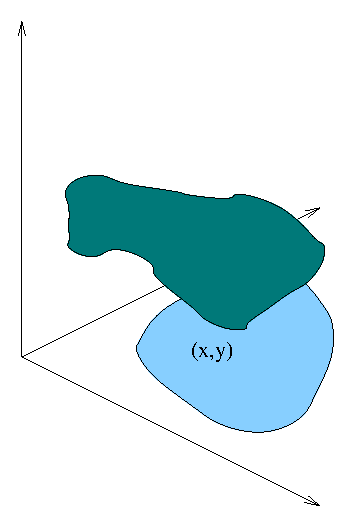
\includegraphics[bb=48 100 150 160,scale=0.8]{an7-1-1.eps}
  Láttuk: egy ``jó'' $g\in\R^2\to\R^1$ fv. képe a térben egy felület.\\
  $\F = \{ (\,x,\,y,\, g(x,y)\,)\in\R^3  \mid (x,y)\in D_g \} \subset \R^3$\\
  ``jó'' függvény esetén ez egy felület.
  
  Szokás: $z=g(x,y)$ egyenlettel adott felület.
  
  Pl. 1. \begin{enumzjb}
  \item sík
  \item félgömb
  \item kúp $g(x,y) := \sqrt{x^2+y^2}\quad ((x,y)\in\R^2)$
  \end{enumzjb}
\item $G(x,y,z)= 0$ implicit megadási mód
  
  pl. gömbfelület.
  \begin{gather*}
    (x,y,z):\quad x^2+y^2+z^2 = R^2\\
    \F = \{ (x,y,z) \mid x^2+y^2+z^2=1\}
    G(x,y,z) := x^2+y^2 + z^2 - 1 = 0
  \end{gather*}
  
\item Kétparaméteres (v. Gauss-féle) megadási mód
  
  \noindent $1.$ pl. gömbfelület ($\F$)
  \begin{gather*}
    x = R \sin v \cos u\\
    y = R \sin v \sin u\\
    z = R \cos v\\
    0 \leq u \leq 2\pi,\quad 0 \leq v \leq \pi
    \intertext{Tehát:}
    F\in\R^2\to\R^3\\
    F(u,v) := \begin{bmatrix}R \sin v \cos u\\
      R \sin v \sin u\\
      R \cos v \end{bmatrix}\qquad(u,v) \in [0,\,2\pi]\times [0,\,2\pi]\\
    \F = R_F
  \end{gather*}

  \noindent $2.$ pl. hengerfelület
  \begin{gather*}
    x = a \sin u\\
    y = a \cos u\\
    z = v\\
    0 \leq u \leq 2\pi,\quad v\in\R
    \intertext{Tehát:}
    F\in\R^2\to\R^3\\
    F(u,v) := \begin{bmatrix}a \sin u\\
      a \cos u\\
      v \end{bmatrix}\qquad(u,v) \in [0,\,2\pi]\times \R\\
    \F = R_F
  \end{gather*}
  
  vö görbe: egy paraméter elég\\
  pl. kúp felületét param. megadni hf.
  
\end{enumerate}

\subsubsection{A felület értelmezése}
\begin{megj} Elsősorban paraméteres megadás.

  Ehhez jelölések
  \begin{gather*}
    I_1,\, I_2 \subset \R \text{ intervallum (bármilyen)}\\
    I_1\times I_2 =: \I^2\subset \R^2 \text{ intervallum}\\
    F\colon \I^2\to\R^3\\
    F=(F_1,\,F_2,\,F_3)\quad F_i\colon \I^2\to\R\text{ koordináta-fv}\\
    \Folyt \text{ - folytonos függvények halmaza}\\
    \Folyt^r \text{ - $r$-szer folytonosan diffható fv-ek halmaza}\\
    \Folyt^0 := \Folyt
  \end{gather*}
\end{megj}

\begin{de}
  $\Folyt^r(\I^2,\,\R^3) \owns F :\ekviv $
  \begin{enumzjr}
  \item $F\colon \I^2\to \R^3$
  \item $F\ $-szer folytonosan deriválható, $r=0,1,2,\ldots$
  \end{enumzjr}
\end{de}

\begin{gather*}
  w := (u,v) \in \I^2 = I_1\times I_2\\
  F'(u,v) = F'(w) = \begin{bmatrix}
    \dfrac{\partial F_1}{\partial u}(w) &  \dfrac{\partial F_1}{\partial v}(w)\\
    \dfrac{\partial F_2}{\partial u}(w) &  \dfrac{\partial F_2}{\partial v}(w)\\
    \dfrac{\partial F_3}{\partial u}(w) &  \dfrac{\partial F_3}{\partial v}(w)\\
  \end{bmatrix} =: \begin{bmatrix}\partial_uF(w) & \partial_vF(w) \end{bmatrix} =:
  \begin{bmatrix}\partial_1F(w) & \partial_2F(w) \end{bmatrix}
\end{gather*}

\begin{de}[Egyszerű, sima felületdarab] Az $\F\subset\R^3$ halmaz egyszerű, sima felületdarab (\textit{ESF}), ha
  $\exists F\in\Folyt^1(\I^2,\R^3)$, melyre
  \begin{enumzjr}
    \item $F\colon \I^2\to\F$ bijekció
    \item $\rang F'(w) = 2 \quad(\forall w\in\I^2)$
  \end{enumzjr}
  Ekkor: az $F$ fv. az $\F$ felület egy paraméterezése.
\end{de}

\begin{Megj}
  \item $\rang F'(w)=2 \ekviv \partial_uF(w), \, \partial_vF(w)$ lineárisan függetlenek
  \item $\Folyt^1$ helyett sokszor többet: $\Folyt^2,\,\Folyt^3,\ldots$
  \item A \textit{felület} neknk: ESF-ekből áll, pl. kocka. Tovább nem pontosítjuk.
  \item Explicit alakból kétparaméteres alak könnyen:\\ha:
    \begin{gather*}
      g\colon\I^2\to\R\text{ folyt. der.}\\
      \F=\{(x,y,g(x,y))\subset\R^3 \mid (x,y)\in D_g\}
      \intertext{akkor:}
     F\colon I^2\to\R^3\\
     F(u,v):=\begin{bmatrix}u\\v\\g(u,v)\end{bmatrix}\quad((u,v)\in\I^2)\\
     F'(u,v) = \begin{bmatrix}1&0\\ 0&1\\\partial_ug(u,v)&\partial_vg(u,v)\end{bmatrix}
    \end{gather*}
    lineárisan függetlenek
\end{Megj}

\subsubsection{Különböző paraméterezések}
$\F\subset\R^3$ ESF, $F\colon \I^2\to\R^3$ egy paraméterezés.

\noindent Legyen: $\J\subset \R^3$ intervallum, $S\colon\J\to\I^2$ $\Folyt^1$-beli bijekció.\\
$G := F\circ S\colon \J\to\F$ az $\F$ felület \emph{egy másik paraméterezése}

\subsection{Határvonalak, felületi görbék}
$\F\subset\R^3$ ESF,  $F\colon \I^2\to\R^3$ egy paraméterezés

\begin{de}[Felületi görbe]%
Az $\I^2$ paramétertarományban fekvő egyszerű, sima síkgörbe $F$ által létesített képét nevezzük
felületi görbének.
\end{de}

\noindent$\gamma\colon[\alpha,\beta]\to\Gamma\subset \I^2$ esg,\\
$\vfi\colon F\circ \gamma\colon [\alpha,\beta]\to\F$ függvénynek értékkészlete egy felületi görbe.


\begin{megj}
  Új jelölés az $\R\to\R^n$ (skalárvektor) függvény deriváltjára:
  \begin{gather*}
    \vfi\colon[\alpha,\beta]\to\R^n\qquad (\vfi(t) := (\vfi_1(t),\dotsc,\vfi_n(t)),\ t\in[\alpha,\beta])\\
    t_0\in[\alpha,\beta]: \Dot{\vfi} := \dfrac{\diff \vfi}{\diff t}(t_0) = \lim_{t\to t_0}\dfrac{\vfi(t)-\vfi(t_0)}{t-t_0}
  \end{gather*}
\end{megj}


\subsection{Érintősík, felületi normális}
\begin{de}[Felületi görbe]%
  $\F\subset\R^3$ ESF, $F\colon \I^2\to\R^3$ egy paraméterezése\\ $[\ F \in\Folyt^1(\I^2,\R^3)\ ]$.\\
  Legyen $\Gamma\subset\F$ egy felületi görbe, $\vfi = F \circ \gamma$ egy par.  \\
  $P_0 = F(u_0,v_0) = (x_0,y_0,z_0)$
\end{de}

\paragraph{A $\Gamma$ görbe érintővektora}%
\begin{gather*}
  \vfi(t_0) = (\Dot{F\circ \gamma})(t_0) = F'(\underbrace{\gamma(t_0)}_{w_0}) \Dot{\gamma}(t_0) = 
  \begin{bmatrix}
    \dfrac{\partial F_1}{\partial u}(w_0) &  \dfrac{\partial F_1}{\partial v}(w_0)\\
    \dfrac{\partial F_2}{\partial u}(w_0) &  \dfrac{\partial F_2}{\partial v}(w_0)\\
    \dfrac{\partial F_3}{\partial u}(w_0) &  \dfrac{\partial F_3}{\partial v}(w_0)\\
  \end{bmatrix} \begin{bmatrix}\Dot{\gamma_1}(t_0) \\ \Dot{\gamma_2}(t_0)\end{bmatrix} =\\ \tag{$\sharp$}\label{eq:sharp}
  = \begin{bmatrix}\partial_uF(w_0) & \partial_vF(w_0) \end{bmatrix} \begin{bmatrix}\Dot{\gamma_1}(t_0) \\
    \Dot{\gamma_2}(t_0)\end{bmatrix} = \Dot{\gamma_1}(t_0) \cdot \partial_uF(u_0,v_0) + \Dot{\gamma_2}(t_0) \cdot
  \partial_vF(u_0,v_0)    
\end{gather*}

\begin{megj}
  A $\partial_uF(u_0,v_0)$, $\partial_vF(u_0,v_0)$ vektorok minden, a $P_0$ ponton átmenő reguláris görbére
  ugyanazok. Ezért minden sima felületi görbe $P_0$-beli érintői ugyanabban a síkban vannak: \textbf{érintősik}.
\end{megj}

\begin{te}%
  $\F\subset\R^3$ ESF, $F\colon \I^2\to\R^3$ egy paraméterezése\\
  $(u_0,v_0)\in\I^2$ rögzített; $P_0:= F(u_0,v_0) = (x_0,y_0,z_0)\in\F$ a megfelelő felületi pont. Ekkor
  \begin{enumerate}
    \item $\forall\ P_0$-on átmenő reguláris (azaz egyszerű, sima) felületi görbe érintői egy síkban vannak. Ezt a síkot
    a felület \textbf{\boldmath $P_0$ pontbeli érintősíkjának} nevezzük.
    \item A felület $P_0$ pontbeli érintősíkjának
      \begin{enumzjb}
      \item \textit{egy bázisa}: $\partial_uF(u_0,v_0),\,\partial_vF(u_0,v_0)\in\R^3$ lineárisan független vektorok
      \item \textit{egy normálvektora}:
	\[ \vekt{m}(u_0,v_0) :=
	\dfrac{\partial_uF(u_0,v_0)\times\partial_vF(u_0,v_0)}{|\partial_uF(u_0,v_0)\times\partial_vF(u_0,v_0)|} \]
	a \textbf{felületi normális egységvektor}, mely az érintősík egy normálvektora
	\item Egyenlete:
	  \begin{gather*}
	    0 = \skalar{x-\underbrace{F(u_0,v_0)}_{(x_0,y_0,z_0)}}{\vekt{m}(u_0,v_0)} \overset{\text{vegyesszorzat}}{=}\\ 
	    = (x-F(u_0,v_0)) \cdot\partial_uF(u_0,v_0) \cdot\partial_vF(u_0,v_0) =\\
	    = \det \begin{bmatrix}x-x_0 & y-y_0 & z-z_0 \\
	    \dfrac{\partial F_1}{\partial u}(u_0,v_0) & \dfrac{\partial F_2}{\partial u}(u_0,v_0) &
	    \dfrac{\partial F_3}{\partial u}(u_0,v_0)\\
	    \dfrac{\partial F_1}{\partial v}(u_0,v_0) & \dfrac{\partial F_2}{\partial v}(u_0,v_0) &
	    \dfrac{\partial F_3}{\partial v}(u_0,v_0)
	    \end{bmatrix} = 0
	  \end{gather*}	  
      \end{enumzjb}
  \end{enumerate}  
\end{te}

\begin{biz}%
  Trivi
\end{biz}

\begin{megj}
  Vegyesszorzat: $\vekt a,\vekt b,\vekt c\in\R^3$
  \[ \vekt{abc} = \skalar{\vekt a}{\vekt{b}\times\vekt c} = \det\begin{bmatrix}
    \mathrm a_x & \mathrm a_y & \mathrm a_z \\ \mathrm b_x & \mathrm b_y & \mathrm b_z \\ \mathrm c_x & \mathrm c_y &
    \mathrm c_z \end{bmatrix}\]
\end{megj}

\begin{te}%
  Tfh. $\F\subset\R^3$ ESF
  \begin{enumzjb}
  \item explicit alakban: $z=g(x,y)\qquad g\in\R^2,\,g\in\Folyt^1$
  \item implicit alakban: $G(x,y,z) = 0\qquad G\in\R^3\to\R^2,\ G\in\C^1,\ldots$
  \end{enumzjb}
  Ekkor:\\
  $\forall P_0=(x_0,y_0,z_0)\in\F$ pontban van érintősík. Ennek egy $\vekt m(P_0)$ \emph{normálvektora},
  ill. \emph{egyenlete}
  \begin{enumzjr}
  \item esetén:
    \begin{gather*}
      \vekt m(P_0) = (\partial_xg(x_0,y_0), \partial_yg(x_0,y_0),-1)\text{, ill.}\\
      z-z_0 = \partial_xg(x_0,y_0)(x-x_0) + \partial_yg(x_0,y_0)(y-y_0)      
    \end{gather*}

  \item esetén:
    \begin{gather*}
      \vekt m(P_0) = (\partial_xG(x_0,y_0,z_0),\partial_yG(x_0,y_0,z_0),\partial_zG(x_0,y_0,z_0))\text{, ill.}\\
      \partial_xG(x_0,y_0,z_0)(x-x_0) + \partial_yG(x_0,y_0,z_0)(y-y_0) +\partial_zG(x_0,y_0,z_0)(z-z_0) =0
    \end{gather*}    
\end{enumzjr}  
\end{te}
\newpage
\begin{biz}
  \begin{enumzjr}
  \item eset:
    \begin{gather*}
      F(u,v) = \begin{bmatrix} u \\ v \\ g(u,v) \end{bmatrix} \text{ egy paraméterezés;}\\
      \partial_u F(u_0,v_0) = \begin{bmatrix} 1 \\ 0 \\ \partial_u g(u_0,v_0) \end{bmatrix} \\
      \partial_v F(u_0,v_0) = \begin{bmatrix} 0 \\ 1 \\ \partial_v g(u_0,v_0) \end{bmatrix}
      \intertext{A sík egy normálvektora:}
      \partial_u F(u_0,v_0) \times \partial_v F(u_0,v_0) = \det \begin{bmatrix} \vekt i & \vekt j & \vekt k \\
	1 & 0 & \partial_1 g(u_0,v_0) \\0 & 1 & \partial_2 g(u_0,v_0) \end{bmatrix}= \begin{bmatrix} -\partial_1g(u,v)
	\\  -\partial_2g(u,v) \\ 1 \end{bmatrix}
    \end{gather*}
    \item eset:
      \begin{gather*}
	G(x,y,z) = 0,\quad \partial_zG(x_0,y_0,z_0) \neq 0
	\intertext{Implicit fv. tétel alkalmazható:}
	\exists g(x,y) : G(x,\,y,\,g(x,y)) = 0\\
	\nn \partial_xG(x,\,y,\,g(x,y)) \cdot 1 + \partial_zG(x,\,y,\,g(x,y)) \cdot \partial_xg(x,y) = 0\\
	\nn \partial_g(x_0,y_0) = - \dfrac{\partial_xG(x,\,y,\,g(x,y))}{\partial_zG(x,\,y,\,g(x,y)} = 0
      \end{gather*}
  \end{enumzjr}
\end{biz}

\subsection{Felületi görbék ívhossza. A felület első alapformája}
$\F\subset\R^3$ ESF, $F\colon \I^2\to\R^3$ egy paraméterezése\\
$\Gamma\subset\F$ egy \textbf{felületi görbe}, $\vfi = \F\circ\gamma\colon [\alpha,\beta]\to\R^3$ egy par.

Mivel $\vfi\in\Folyt^1([\alpha,\beta],\,\R^3)$, ezért $\Gamma$ rektifikálható, és az ívhossza:
\[ l_\Gamma = \Int_\alpha^\beta \vert \Dot{\vfi}(t)\vert \diff t =  \Int_\alpha^\beta 
\sqrt{\Dot{\vfi_1}^2(t) + \Dot{\vfi_2}^2(t) + \Dot{\vfi_3}^2(t)}\diff t\]
      
Kérdés: $l_\Gamma$-t az $F$-fel és a $\gamma$-val kifejezni:

Válasz:
\begin{gather*}
   \eqref{eq:sharp} \nn \Dot\vfi(t)=\Dot{\gamma_1}(t)\partial_uF(u,v) + \Dot{\gamma_2}(t)\partial_vF(u,v)\\
   \hspace*{2cm}(\vfi(t) = (u,v))
  \intertext{\underline{Vagy}}
  \Dot\vfi=\Dot{\gamma_1}\partial_uF + \Dot{\gamma_2}\partial_vF\\
  \intertext{Ezért:}
  |\Dot\vfi|^2=\skalar{\Dot\vfi}{\Dot\vfi} = 
  \skalar{\Dot{\gamma_1}\partial_uF + \Dot{\gamma_2}\partial_vF}{\Dot{\gamma_1}\partial_uF + \Dot{\gamma_2}\partial_vF}=
  \\ =\Dot{\vfi_1}^2\underbrace{\underbrace{\skalar{\partial_uF}{\partial_vF}}_{\eE} + 
  2\Dot{\vfi_1}\Dot{\vfi_2}\underbrace{\skalar{\partial_uF}{\partial_vF}}_{\eF} +
  \Dot{\vfi_2}^2\underbrace{\skalar{\partial_vF}{\partial_vF}}_{\eG}}_{
    \text{A Gauss-féle első alapkmennyiségek}}
\end{gather*}

\begin{de}[A Gauss-féle első alapmennyiségek]%
  Pontról pontra változnak:
  \begin{gather*}
    t_0\in[\alpha,\beta],\ \gamma(t_0)=(u_0,v_0)=w_0\\
    \eE = \eE(t_0) = \eE(w_0) :=\skalar{\partial_uF(w_0)}{\partial_uF(w_0)}\\
    \eF = \eF(t_0) = \eF(w_0) :=\skalar{\partial_uF(w_0)}{\partial_vF(w_0)}\\
    \eG = \eG(t_0) = \eG(w_0) :=\skalar{\partial_vF(w_0)}{\partial_vF(w_0)}
  \end{gather*}  
\end{de}
\begin{Megj}
\item Kvadratikus alak: 
  \begin{gather*}
    A = \begin{bmatrix} a & b \\ c & d \end{bmatrix}\\
    Q(\vekt x) = Q(x_1,x_2) = \skalar{A\vekt x}{\vekt x} = ax_1^2 + 2bx_1x_2 + cx_2^2
  \end{gather*}
\item  $G(w) = \begin{bmatrix} \eE(w) &\eF(w)\\ \eF(w) &\eG(w) \end{bmatrix} = \begin{bmatrix} g_{ij}(w) \end{bmatrix}
  \quad w = (u,v)$  
  
  \noindent Ezzel: $\left\vert \Dot\vfi(t) \right\vert^2 = \skalar{G(\gamma(t))\cdot\Dot\gamma(t)}{\Dot\gamma(t)}$
  
  \noindent A $\Gamma$ görbe ívhossza:
  \begin{gather*}
    l_\Gamma = \Int_\alpha^\beta \sqrt{ \skalar{G(\gamma(t))\cdot\Dot\gamma(t)}{\Dot\gamma(t)}}\diff t = \\
    = \Int_\alpha^\beta \sqrt{ \eE(t)\Dot{\vfi_1}^2(t) + 2\eF(t)\Dot{\vfi_1}(t)\Dot{\vfi_2}(t) +
      \eG(t)\Dot{\vfi_2}^2(t)} \diff t\\ \left(= \Int_\alpha^\beta \sqrt{\eE\Dot{\vfi_1}^2 + 2\eF\Dot{\vfi_1}\Dot{\vfi_2}
      + \eG\Dot{\vfi_2}^2}\diff t\right)    
\end{gather*}
\end{Megj}

\begin{de}[Első alapforma]
  Legyen $\F\subset\R^3$ ESF, $F\colon \I^2\to\R^3$ egy paraméterezése; $w=(u,v)\in\I^2$. A
  \[ G(w) = \begin{bmatrix} \eE(w) &\eF(w)\\ \eF(w) &\eG(w) \end{bmatrix} \]
  szimmetrikus mátrix-szal kézett
  \[  Q(\vekt x) = Q(x_1,x_2) = \skalar{G(w)\vekt x}{\vekt x} = \eE(w)x_1^2 + 2\eF(w)x_1x_2 + \eG(w)x_2^2\]
  kvadratikus alakot a felület \emph{első alapformájának} nevezzük.  
\end{de}

\begin{te}
  A $Q(x_1,x_2)$ kvadratikus alak pozitív definít, azaz
  \[ Q(x_1,x_2) > 0\ \forall \vekt x=(x_1,x_2) \in\R^2\setminus \{(0,0)\} \]
  mert
  \[ \eE(w) > 0,\ \det G(w) = \eE(w)\eG(w) - \eF^2(w) = | \partial_uF(w) \times\partial_vF(w) | >0
  \quad (\forall w\in\I^2)\]
\end{te}

\begin{biz}
  \begin{gather*}
    \eE(w) :=  \partial_uF(w) \cdot \partial_uF(w)> 0\quad \text{skaláris szorzat}\\
    \eE\eG - \eF^2 = (\partial_uF \cdot \partial_uF)\left(\partial_vF \cdot \partial_vF\right) - 
    (\partial_uF \cdot \partial_vF)^2 =\\
    = |\partial_uF|^2|\partial_vF|^2 - |\partial_uF|^2 \cdot |\partial_uF|^2 \cdot \cos^2 \alpha =  
    |\partial_uF|^2|\partial_vF|^2 \cdot \sin^2\alpha =  |\partial_uF\times\partial_vF|^2 > 0
  \end{gather*}
\end{biz}



\subsection{Felületek felszíne}
(Motiváció)
\begin{de}[Felület felszíne]
  $\F\subset\R^3$ ESF, $F\colon \I^2\to\R^3$ egy par.\\
Ekkor az $\F$ felszíne:
\[ \fel := \fel_\F := \Iint_T\!|\partial_uF(u,v) \times \partial_vF(u,v)| \diff u \diff v \]  
\end{de}

\begin{te}
  A definíció független a paraméterezéstől.
\end{te}


\subsubsection{A felszín kiszámolása}

\begin{te}
  $\F\subset\R^3$ ESF
\begin{enumzjr}
\item ha $F\colon\I^2\to\R^3$ egy par., akkor
  \[ \fel = \Iint_T\!\sqrt{\eE\eG-\eF^2}\diff u \diff v\]
\item ha $\F$: $z=g(x,y)$ explicit alak; $(x,y)\in T$, akkor
  \[ \fel = \Iint_T\!\sqrt{1+g^2_x + g^2_y} \diff u \diff v\]
  ahol $g_x$, $g_y$ az $x$, $y$ változó szerinti parciális derivált.
\item Ha $\F$: $G(x,y,z) = 0$ implicit alak
  \[ \fel = \Iint_T \dfrac{\sqrt{G_x^2 + G_y^2 + G_z^2}}{|G_z|}\diff u \diff v\]\end{enumzjr}
\end{te}

\begin{biz}
  \begin{enumzjr}
  \item poz. def.-re vonatkozó tétel alapján.
  \item%
    \begin{gather*}
      F(u,v) := \begin{bmatrix} u\\ v \\ g(u,v) \end{bmatrix}\\
      \partial_uF(u,v) = \begin{bmatrix} 1\\ 0 \\ \partial_ug(u,v) \end{bmatrix}\qquad
      \partial_vF(u,v) = \begin{bmatrix} 0\\ 1 \\ \partial_vg(u,v) \end{bmatrix}\\
      \left.\begin{array}{l}\eE = \partial_uF \cdot \partial_uF = 1 + g_u^2\\
      \eF = \partial_uF \cdot \partial_vF = g_u \cdot g_v\\
      \eG = \partial_vF \cdot \partial_vF = 1 + g_v^2\end{array}\right\}
      \nn \eE\eG-\eF^2 = 1 +g_v^2 + g_v^2
    \end{gather*}
    \item feltesszük, hogy az egyik változó kifejezhető, pl. a 3.
      \begin{gather*}
	G(x,y,z) = 0 \nn \exists g(x,y) : G(x,\,y,\,g(x,y)) = 0 ;\  G_z\neq 0\\
	\nn g_x = \dfrac{-G_x}{G_z}\quad g_y = \dfrac{-G_y}{G_z}
      \end{gather*}      
  \end{enumzjr}
\end{biz}

\begin{megj}
  Forgástest felszíne:
  \[ \fel = 2\pi\Int_a^bf(x)\sqrt{1+[f'(x)]^2}\diff x\]
  Ugyanis: 
  \begin{gather*}
    y=f(x);\ \F : y^2 + z^2 =  f(x)\\
    G(x,y,z) = y^2 + z^2 - f(x)      
  \end{gather*}
  Erre (c)-t alkalmazva adódik a képlet.
\end{megj}


\subsection{Második alapmennyiségek}
\begin{megj}
  Az első alapmennyiségek: $\eE,\,\eF,\,\eG$ a felület \emph{metrikus tulajdonsáihoz} kapcsolhatóak.\\
  A második alapmennyiségek a felület \emph{alakjával} kapcsolatosak.
\end{megj}

\noindent $\F\subset\R^3$ ESF, $F\colon \I^2\to\R^3$; $F\in\Folyt^2(\I^2,\R^3)$\\
$\F\owns P_0=F(w_0) = F(u_0,v_0)$;  $F$-re Taylor-formulából; $h=(h_1,h_2)\in\R^2$

\begin{gather*}
  F(w_0+h) = F(w_0) + \partial_uF(w_0)\cdot h_1 + \partial_vF(w_0)\cdot h_2 + {}\\
  {}+ \dfrac12 \left[ \partial_{uu}F(w_0)\cdot h_1^2 + 2\partial_{uv}F(w_0)\cdot h_1h_2\partial_{uv}F(w_0)\cdot h_2^2
  \right] +  \underbrace{R(w_0,h)\cdot |h|^2}_{\text{maradéktag}} =\\
  =T(h) + R(w_0,h)\cdot |h|^2\\
  T(h) = T_{F,w_0,2}(h)
\end{gather*}

A maradéktag tart nullához, ha $h\to0$


Pont és sík távolsága: $\dist(P,\epsilon) = \skalar{\vekt r - \vekt{r_0}}{n_0}$, $P=T(h)$
\begin{gather*}
  \dist(P,\epsilon) = \dist(T(h),\epsilon) = \skalar{T(h)-F(w_0)}{\vekt m(w_0)}
  \overset{\partial_uF\perp \vekt m}{\underset{\partial_vF\perp \vekt m}{=}}\\
  = \dfrac12 [\,\underbrace{\underbrace{\partial_{uu}F(w_0)\cdot\vekt m(w_0)}_{\mL(w_0)}h_1^2 + 
      2\underbrace{\partial_{uv}F(w_0)\cdot\vekt m(w_0)}_{\mM(w_0)}h_1h_2 +
      \underbrace{\partial_{vv}F(w_0)\cdot\vekt m(w_0)}_{\mN(w_0)}}_{
      \text{Gauss-féle 2. alapmennyiségek a } P = F(w_0) \text{ pontban}}h_2^2  \,]\\
  H(w) := \begin{bmatrix} \mL(w) &  \mM(w) \\  \mM(w) &  \mN(w) \end{bmatrix}
  \intertext{A felület második alapformája a $P=F(w)$ pontban:}
  Q(h) := \skalar{H(w)\cdot \vekt h}{\vekt h}
\end{gather*}

\begin{megj}
  $\dist(P,\epsilon) = \dfrac12\skalar{H(w_0)\vekt h}{\vekt h}$
\end{megj}



\subsection{Felületi görbék görbülete. Felületi pontok osztályozása}


\subsubsection{Felületi görbék görbülete}
$\F\subset\R^3$ ESF, $F\colon \I^2\to\R^3$ egy paraméterezése; $\Gamma\subset\F$ felületi görbe;
$\vfi=F\circ\gamma$; $P_0\in\F$\\
$\kappa(P_0) = |\Phi''(s_0)|$; $\Phi=\vfi\circ T= F\circ\gamma\circ T$

\begin{te}
  $\F\subset\R^3$ ESF, $F\colon \I^2\to\R^3$ egy paraméterezése; $\Gamma\subset \F$ fel. görbe,\\ $\vfi =
  F\circ\gamma\colon[\alpha,\beta]\to\F$ param; $P_0\in\F$, $P_0 = F(\gamma(t_0))=F(u_0,v_0)=F(w_0)$.
  Ekkor
  \begin{gather*}
    \kappa(P_0)=\dfrac1{\vekt n(P_0) \cdot\vekt m(w_0)}\cdot\dfrac{\skalar{H(w_0)\cdot
	\Dot\gamma(t_0)}{\Dot\gamma(t_0)}}{\skalar{G(w_0)\cdot \Dot\gamma(t_0)}{\Dot\gamma(t_0)}} = \tag{$*$}\label{eq:*}\\
    = \dfrac1{\vekt n(P_0) \cdot\vekt m(w_0)} \cdot
    \dfrac{\mL(w_0)\Dot{\gamma_1}^2(t_0) +2\,\mM(w_0)\Dot{\gamma_1}(t_0)\Dot{\gamma_2}(t_0)
      +\mN(w_0)\Dot{\gamma_2}^2(t_0)}{\eE(w_0)\Dot{\gamma_1}^2(t_0) +2\,\eF(w_0)\Dot{\gamma_1}(t_0)\Dot{\gamma_2}(t_0)
      +\eG(w_0)\Dot{\gamma_2}^2(t_0)}
  \end{gather*}
  ha $\vekt n \cdot \vekt m \neq 0$ azaz az érintősík $\not\equiv$ a görbe simulósíkja
\end{te}

\begin{Megj}
  \item $\vekt n(P_0)$ a görbe főnormális egységvektora\\
    $\vekt m (w_0)$ a felület normálisa
  \item A tétel gyakorlati haszna: $\kappa(P_0)$ számolható. Fontosabb: \emph{elméleti jelentősége}:
    $\kappa(P_0)$ nem változik akkor, ha végigosztjuk $\gamma_2^2$-tel (alul, felül). Tehát csak kettő értéktől függ:
    \begin{itemize}
      \item $\dfrac{\gamma_1(t_0)}{\gamma_2(t_0)}$ hányadostól; az érintőiránytól - a paramétertartományban egy irányt ad
	meg, mely meghatároz az érintősíkban egy irányt
      \item $\vekt n(P_0)$-tól.
    \end{itemize}
   
    Ezek szerint az azonos érintővel és simulósíkkal rendelkező görbék görbülete ugyanaz. $\nn$ Fel. görbék vizsgálata:
    elég a síkmetszeteket (síkmetszetek görbületét) vizsgálni, mert tertszőleges görbe $P_0$-beli görbülete = a görbe
    simulósíkja által a felületből kimetszett görbe görbületével.
\end{Megj}


\begin{de}\ \\
  \emph{Normálsík}: $P_0$-ban az érintősíkra merőleges.\\
  \emph{Normálmetszet}: amit a normálsík a felületből kimetsz. Ennek görbülete: \emph{normálgörbület}
  \emph{Ferdemetszet}: a többi síkmetszet
\end{de}

\begin{megj}
  $\eqref{eq:*}\nn$ \emph{normálmetszet}et elég vizsgálni: $\vekt n\Vert \vekt m\nn \vekt n \cdot \vekt m = \pm 1$
\end{megj}


\begin{de}[Előjelezett normálgörbület] (ld. \ref{eq:*}.) $e$ egy irány az érintősíkban:
  \[ \kappa_e(P_0) := \dfrac{\skalar{H(w_0)\Dot{\gamma}(t_0)}{\Dot\gamma(t_0)}}{
    \skalar{G(w_0)\Dot{\gamma}(t_0)}{\Dot\gamma(t_0)}} \]
\end{de}

\begin{megj}
  Világos (\ref{eq:*}): $\kappa_e(P_0) > 0$, ha $\vekt n$ és $\vekt m$ egyirányú;\\
  $\kappa_e(P_0) < 0$, ha $\vekt n$ és $\vekt m$ ellentétes irányú.
\end{megj}

\begin{te}[Meusnier tétele ferdemetszetekről]
  $\sigma$ egy ferdemetszet, az érintősík $\vekt e$ egyenese irányában.
  $\kappa (P_0)$ a ferdemetszet görbülete.\\
  \[\kappa(P_0) = \dfrac{\kappa_e(P_0)}{\cos\alpha}\qquad \alpha\in(0,\pi)\setminus\{\dfrac\pi2\}\]
  $\alpha$ a síkok hajlásszöge: $\vekt n$ és $\vekt m$ szöge ($\vekt n \cdot \vekt m \neq 0$)  
\end{te}

\newpage
\begin{Megj}
\item Elég a normálmetszetek görbületét ismerni
\item további teendő: az érintősíkban különbözö irányokban az arra $\perp$ síkmetszetek görbületét vizsgálni:
  azaz $\kappa_e(P_0)$ viszgálata; hogyan változik a kül. irányokban.
\item Dallam: Az érintősíkban van 2 egymásra merőleges irány (\emph{főirányok}), amelyek (görbületek) ismeretében minden
  irányú normálgörbület meghatározható (Euler-tétel)
\end{Megj}


\subsubsection{Egy általános szélsőértékfeladat}

\begin{te}
  Legyen
  \[ f(x) := \dfrac{\skalar{\vekt A\vekt x}{\vekt x}}{\skalar{\vekt B\vekt x}{\vekt x}} \quad (\vekt x\in\R^n\setminus
  \{0\}) \]
  ahol $\vekt A,\vekt B\in\R^{n\times n}$ szimmetrikus; $\vekt B$ poz. definit ($\det \neq 0 \nn \exists$ inverz)\\
  Tekintsük az $\vekt A\cdot\vekt B^{-1}$ szimm. mátrixot, jelöljük:\\
  $\lambda_1 \leqq \lambda_2 \leqq\ldots \leqq   \lambda_n$ a sajátértékek,\\
  $\vekt {r_1},\vekt{r_2},\dotsc, \vekt{r_n}$ a sajátvektorok\\
  Ekkor:
  \begin{enumzjr}
  \item $f$-nek $\exists$ absz. min., absz. max. (folyt., konv.)
  \item $\min f = \lambda_1 \overset{\text{sőt!}}{=} f(B^{-1}\vekt r_1)$ absz. min.\\
    $\max f = \lambda_n =  f(B^{-1}\vekt r_1)$    
\end{enumzjr}
\end{te}

\begin{Megj}
\item $f$ folyt., homogén (skalárral szorozva nem változik); kör mentén azonos értékeke
\item biz: (i) trivi, (ii) biz nélkül.
\item alkalmazás: $A := H(w_0),\ B:=G(w_0)\in\R^{2\times2}$\\
  $\vekt x=(x_1,x_2)$ az érintősíkban az $e = x_1\partial_uF(w_0) + x_2 \partial_vF(w_0)$ irányt hat. meg

  Itt a $\partial_uF(w_0)$, $\partial_vF(w_0)$: az érintősík bázisvektorai.
\end{Megj}


\begin{te}[Főgörbületekre]
  $\F\subset\R^3$ ESF, $F\colon \I^2\to\R^3;\ F\in \Folyt^3$ egy paraméterezése; $P_0=F(w_0)\in\F$
  \begin{enumzjr}
  \item Ekkor az
    \begin{gather*}
      f(x):= \kappa_e(P_0) = \dfrac{\skalar{H(w_0)\vekt x}{\vekt x}}{\skalar{G(w_0)\vekt x}{\vekt x}} = \\
      = \dfrac{\mL(w_0)x_1^2 + 2\,\mM(w_0)x_1x_2 + \mN(w_0)x_2^2}{\eE(w_0)x_1^2 + 2\,\eF(w_0)x_1x_2 + \eG(w_0)x_2^2}
      \quad x=(x_1,x_2)\in\R^2\setminus\{\vekt 0\}
    \end{gather*}
    fv-nek $\exists$ absz. minimuma ($\kappa_1$) és absz. maximuma ($\kappa_2$).\\Ezek az ún. \emph{fő(normál)görbületek}
  \item $\kappa_1, \kappa_2$: a $H(w_0)G^{-1}(w_0) \in\R^{2\times2}$ mátrix sajátértékei
  \item $\kappa_1+\kappa_2 = \tr(H(w_0) G^{-1}(w_0) =: \mathcal{H}\quad $ \emph{összeggörbület} (Minkovszki-féle görbület)\\
    $\kappa_1\cdot\kappa_2 = \det{H(w_0) G^{-1}(w_0)} =: \mathcal{K}\quad $ \emph{szorzatgörbület} (Gauss-féle görbület)
    
  \item A főgörbületek tehát a
    \[ \lambda^2 - \tr(H(w_0)G^{-1}(w_0)) + \det(H(w_0)G^{-1}(w_0)) = 0 \tag{$\approx$}\label{eq:fogorbSE}\]
    sajátértékegyenlet gyökei (mindig valósak)
  \end{enumzjr}  
\end{te}

\begin{te}
  $A=[a_{ij}]\in\R^{n\times n}$
  \[ \tr(A) := \sum_{k=1}^n a_{kk}\]
  az $\vekt A$ mátrix nyomának nevezzük
\end{te}

\begin{megj}
  A főgörbületek meghat.
  \begin{enumerate}
    \item $H(w_0)$, $G(w_0)$ számolása
    \item $H(w_0)$, $G^{-1}(w_0)$ számolása
    \item \eqref{eq:fogorbSE} felírása, megoldás
  \end{enumerate}
  $\nn \kappa_1,\,\kappa_2$
\end{megj}


\begin{te}[Főirányok]
  Az előző tételbeli $f$ fv. szélsőértékhelyei és az érintősíkban $(\xi,\eta)$ koordinátákat határoz meg a
  \[ \xi\partial_uF(w_0) + \eta\partial_vF(w_0)\]
  alapján. Ezek az ún. \emph{főirányok}

  {\listaszamkor
    \begin{enumerate}
    \item Ha $\kappa_1\neq \kappa_2 \nn$ két főirány van és ezek merőlegesek egymásra
      Ha $\kappa_1= \kappa_2 \nn$ minden főirány (pl. gömb)
    \item A főirányokat megadó $\xi,\,\eta$ értékek a
      \[ \det \begin{bmatrix} \eta^2 & -\xi\eta & \xi^2\\
	  \eE(w_0) &\eF(w_0) &\eG(w_0) \\ \mL(w_0) &\mM(w_0) &\mN(w_0) &  \end{bmatrix}\] = 0
    \end{enumerate}

  }
\end{te}
\begin{biz}
  nélkül.
\end{biz}

\begin{megj}
  Jól számolható. A $\dfrac{\xi}{\eta}$-ra másodfokú képlet.
\end{megj}

\begin{te}[Euler tétele]
  $\F\subset\R^3$ ESF; $P_0\in\F$; $\sigma$ egy tetszőleges normálmetszet $P_0$-ban. $\kappa$: normálmetszet (görbe)
  görbülete $P_0$-ban.
  Ekkor:
  \[ \kappa = \kappa_1\cos^2\vartheta + \kappa_2\sin^2\vartheta\]
  ahol $\kappa_1,\,\kappa_2$ fő(nromál)görbület, $\vartheta$ az $e$ értintő és $\kappa_1$-nek megfelelő főirány által
  bezárt szög.
\end{te}

\subsubsection{Felületi pontok osztályozása}
\begin{de}
  $\F\subset\R^3$ ESF, $P_0\in\F$, $\mathcal{K} := \kappa_1\cdot\kappa_2$ szorzatgörbület.
  A $P_0$ pont
  \begin{itemize}
  \item \emph{elliptikus}, ha $\mathcal{K} > 0$
  \item \emph{hiperbolikus}, ha $\mathcal{K} < 0$
  \item \emph{parabolikus}, ha $\mathcal{K} = 0$
  \item \emph{szférikus}, ha $\kappa_1 = \kappa_2 \neq 0$
  \item \emph{planáris}, ha $\kappa_1 = \kappa_2 = 0$
  \end{itemize}
\end{de}

\begin{megj}
  Az osztályozás nem diszjunkt. Speciális másodrendű felületeknél ellenőrizni!
\end{megj}

% fill-column: 120
% TeX-master: t
% End:

  \newpage
  \include{vektoranalizis}
%  \newpage
%  \include{mertekelmelet}
\end{document}

% Local Variables:
% fill-column: 120
% TeX-master: t
% End:
